\documentclass[../main.tex]{subfiles}
\graphicspath{{\subfix{../diagrams/}}}


\begin{document}

\chapter{Silicon Implementation}
\section{Synthesis}
%%%%%%%%%%%%%%%%%%%%%%%%%%%%%%%%%%%%%%%%%%%%%%%%%%%%%%%%%%%%%%%%%%%%%%%%%%%%%%%%%%%%%%%%%%%%%%%%%%%%%%
\subsection{Flow chart of the synthesis process}
The logic synthesis process consists of two main steps - translation and 
optimization. See figure \ref{fig:syn_flow} for the complete flow of the synthesis process. Figure \ref{fig:ip_op_syn} illustrates the inputs and outputs of this process.

\begin{itemize}
\item Translation involves transforming a HDL (RTL) description to gates
\item Optimization involves selecting the optimal combination of ASIC technology library cells to achieve the required functionality.
\end{itemize}

\begin{figure}[h]
    \centering
    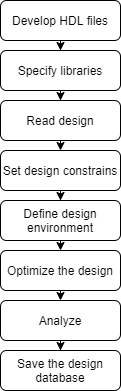
\includegraphics[width=3cm]{diagrams/syn_flow.png}
    \caption{Synthesis flow}
    \label{fig:syn_flow}
\end{figure}

\begin{figure}[h]
    \centering
    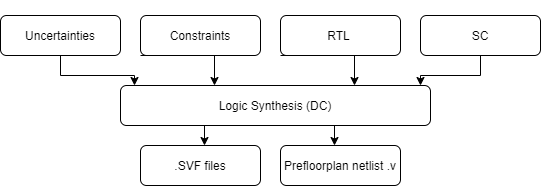
\includegraphics[scale = 0.8]{diagrams/ip_op_syn.png}
    \caption{Input and Output files}
    \label{fig:ip_op_syn}
\end{figure}
%%%%%%%%%%%%%%%%%%%%%%%%%%%%%%%%%%%%%%%%%%%%%%%%%%%%%%%%%%%%%%%%%%%%%%%%%%%%%%%%%%%%%%%%%%%%%%%%%%%%%%
\subsection{Setting the libraries}
The technology library to which the design will be mapped must be defined in order for the synthesis tool to know how to map the design. The following are the many library types, each of which provides particular information on the cells and the technology:

\begin{itemize}
\item \textbf{Technology libraries:} \\
Each cell in a semiconductor vendor's library has information on its features and functions. Cell name, area, delay, function, default design rule restrictions, operating circumstances, and wire-load model are some of the features that may be defined for each cell. DC should be given a technology library in.db format. These libraries are:
    \begin{enumerate}
        \item used by DC as the target library, which contains the cells to which the design will be mapped
        \item part of the link library (along with other sub-designs), which DC uses to resolve references.
        \item used to calculate delay and power consumption of the design, as they contain timing and power information about the cells.
    \end{enumerate}

\item \textbf{Symbol libraries:}\\
They contain the graphic symbols that represent library cells which are used when we want to draw the circuit schematics (in Design Vision). They usually have the extension ".sdb".

\item \textbf{DesignWare libraries:}\\
They contain reusable building blocks or components, that implement specific well-known functions like addition, subtraction, multiplication, and operators like \(>, <, \geq, \leq\).
They usually have the extension ".sldb".
\end{itemize}
%%%%%%%%%%%%%%%%%%%%%%%%%%%%%%%%%%%%%%%%%%%%%%%%%%%%%%%%%%%%%%%%%%%%%%%%%%%%%%%%%%%%%%%%%%%%%%%%%%%%%%
\subsection{Reading in the design}
DC provides us with two different methods:

\begin{itemize}
\item \textbf{Analyse then Elaborate Method:}\\
The analyze and then elaborate method is the preferred method to use when reading in new RTL for various reasons. This method works in two phases, the first phase is the analyze phase where the design is read, checked for any errors and stored as an intermediate result in the default WORK library, or any other library specified by the user.\\
\newline
\noindent The second phase is the elaborate phase where the design is mapped to a GTECH 
implementation and the HDL operators are replaced with the appropriate DesignWare 
components. During this phase it is allowed to select non-default values for design 
parameters, finally DC resolves references and reports if there are any unresolved 
references in the design.

\item \textbf{Read\_file Method:}\\
The read\_file method performs more or less the same functionality of the analyze
and elaborate method, with some differences. The read\_file method works in one stage only so it is less preferable when it comes to reading in new designs, as it does not allow for intermediate results like the analyse command. The read\_file method does not automatically resolve references and report unresolved ones; the user must use link command afterwards to do that
\end{itemize}
%%%%%%%%%%%%%%%%%%%%%%%%%%%%%%%%%%%%%%%%%%%%%%%%%%%%%%%%%%%%%%%%%%%%%%%%%%%%%%%%%%%%%%%%%%%%%%%%%%%%%%
\subsection{Constraints}
The design rule constraints we will be discussing are: maximum transition time, maximum fanout, maximum capacitance and minimum capacitance. 

\begin{itemize}
\item \textbf{Maximum Transition Time:} We use the \textit{set\_max\_transition} command to set the longest time (in time units consistent with those defined in the technology library) required for the driving pin of a net to change its logic value.
\item \textbf{Maximum Fanout:} We use the \textit{set\_max\_fanout} command to set the maximum number of equal gates that can be driven by this port or design. DC attempts to ensure that the sum of fanout\_load attributes of the driven cells is less than the max\_fanout attribute of the driving cell.
\item \textbf{Maximum and Minimum Capacitance:} We use the \textit{set\_max\_capacitance} command to define the maximum total capacitive load that an output port can drive. Capacitance is specified in units consistent with technology library definition
\\Similarly, we use the\textit{ set\_min\_capacitance} command to define the minimum total capacitive load an output port can drive, in units consistent with technology library capacitance units.
\end{itemize}
%%%%%%%%%%%%%%%%%%%%%%%%%%%%%%%%%%%%%%%%%%%%%%%%%%%%%%%%%%%%%%%%%%%%%%%%%%%%%%%%%%%%%%%%%%%%%%%%%%%%%%
\subsection{ Report analysis}
Design Compiler offers us the convenience of generating a wide variety of reports, to validate the correctness and quality of our implementation.

\begin{itemize}
\item \textbf{Timing reports:}\\
Design Compiler has a built-in static timing analyzer called DesignTime. Static Timing Analysis 
can determine if a circuit meets timing constraints without dynamic simulation which is an advantage when it comes to saving time. Seen figure \ref{fig:timing_report}.

\begin{figure}[h!]
    \centering
    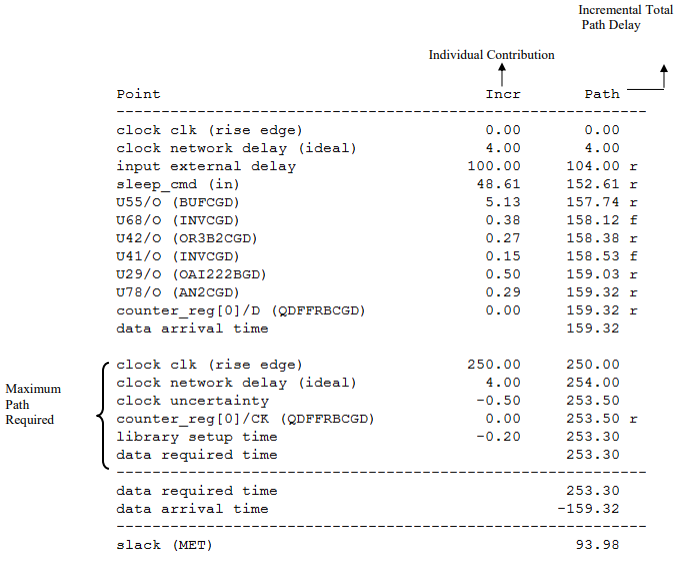
\includegraphics[scale = 0.75]{diagrams/timing_report.PNG}
    \caption{Timing report}
    \label{fig:timing_report}
\end{figure}

\item \textbf{Area reports:}\\
The overall area of the design is included in this report. It estimates this area by combining the area characteristics of the technology library's gates. The area units are usually defined in the technology.also in the library, or in a related document as seen below in figure \ref{fig:area_report}

\begin{figure}[h!]
    \centering
    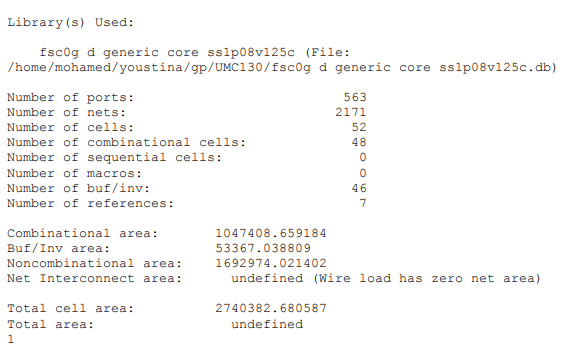
\includegraphics[scale = 0.75]{diagrams/area_report.PNG}
    \caption{Area report}
    \label{fig:area_report}
\end{figure}
\end{itemize}
%%%%%%%%%%%%%%%%%%%%%%%%%%%%%%%%%%%%%%%%%%%%%%%%%%%%%%%%%%%%%%%%%%%%%%%%%%%%%%%%%%%%%%%%%%%%%%%%%%%%%%
\subsection{RISC-V synthesis flow and challenges}
\subsubsection{Script steps:}
\begin{enumerate}
\item  Identify technology library.
\item  Import design (netlist).
\item  Design constraints.
\end{enumerate}
ADD TEXT HERE......................
%%%%%%%%%%%%%%%%%%%%%%%%%%%%%%%%%%%%%%%%%%%%%%%%%%%%%%%%%%%%%%%%%%%%%%%%%%%%%%%%%%%%%%%%%%%%%%%%%%%%%%
%%%%%%%%%%%%%%%%%%%%%%%%%%%%%%%%%%%%%%%%%%%%%%%%%%%%%%%%%%%%%%%%%%%%%%%%%%%%%%%%%%%%%%%%%%%%%%%%%%%%%%
%%%%%%%%%%%%%%%%%%%%%%%%%%%%%%%%%%%%%%%%%%%%%%%%%%%%%%%%%%%%%%%%%%%%%%%%%%%%%%%%%%%%%%%%%%%%%%%%%%%%%%
\section{Physical Design (PnR)}
The goal of physical design is to convert the synthesized netlist into a GDSII file that is 
manufacturable. Figure \ref{fig:PnR_flow} displays the main steps of PnR flow and figure \ref{fig:IO_IC} illustrates the inputs and outputs of the PnR process using IC Compiler.

\begin{figure}[h]
\centering
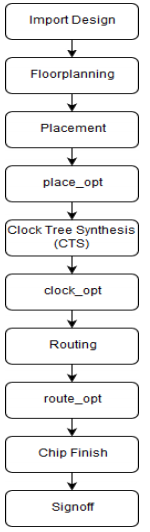
\includegraphics[width=4cm]{diagrams/PnR_flow.PNG}
\caption{Placement and routing flow}
\label{fig:PnR_flow}
\end{figure}

\begin{figure}[h]
\centering
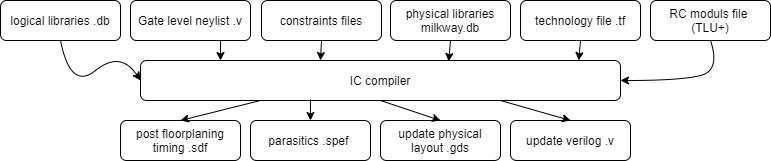
\includegraphics[width=15cm]{diagrams/IO_IC.png}
\caption{ Input and output files for PnR}
\label{fig:IO_IC}
\end{figure}
%%%%%%%%%%%%%%%%%%%%%%%%%%%%%%%%%%%%%%%%%%%%%%%%%%%%%%%%%%%%%%%%%%%%%%%%%%%%%%%%%%%%%%%%%%%%%%%%%%%%%%
\subsection{Floorplanning} 
\subsubsection{Description and basic Concepts}
\begin{enumerate}
\item Size and shape of the block.
\item Voltage area creation (Power domains).
\item IO placement.
\item Creating standard cell rows.
\item Macro-placement.
\item Adding routing and placement blockages (as required).
\end{enumerate}

Inputs and outputs Of this stage are illustrated in Fig \ref{fig:IO_floorplaning}.

\begin{figure}[h]
\centering
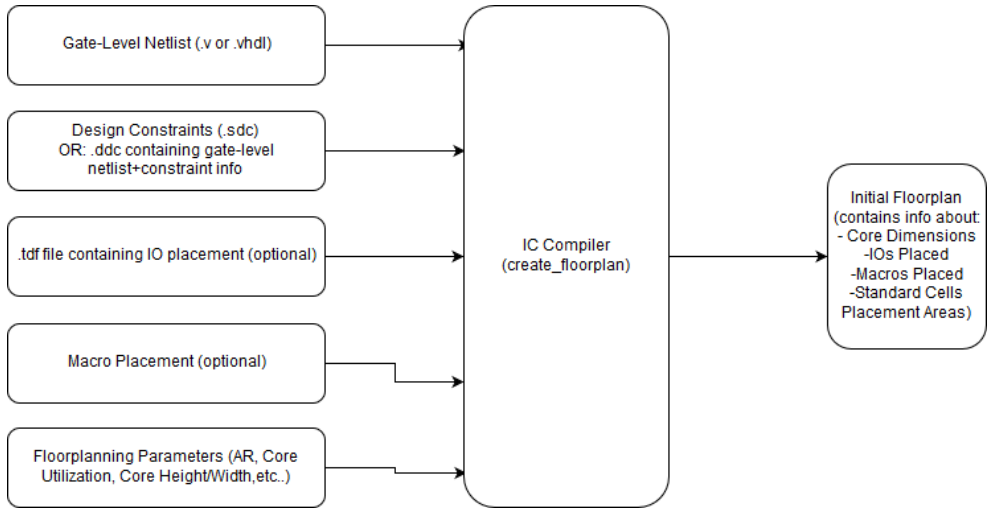
\includegraphics[width=15cm]{diagrams/IO_floorplaning.PNG}
\caption{ Inputs and Outputs of Floorplanning}
\label{fig:IO_floorplaning}
\end{figure}

\subsubsection{Floorplanning Goals}
\begin{enumerate}
\item Minimize the total chip area.
\item Make routing phase easy (routable).
\item Improve the performance by reducing signal delays.
\item Place macros and blocks in the core.
\item Determine routing areas between macros/blocks.
\end{enumerate}
%%%%%%%%%%%%%%%%%%%%%%%%%%%%%%%%%%%%%%%%%%%%%%%%%%%%%%%%%%%%%%%%%%%%%%%%%%%%%%%%%%%%%%%%%%%%%%%%%%%%%%
\subsection{Power-Planning}

\begin{enumerate}
\item  \textbf{Rings:}\\
These are the structures that surround the core and any macro or black box. They carry the VDD/VSS around the chip.
\item \textbf{Stripes:}\\
These structures carries VDD and VSS from Rings across the chip.
\item \textbf{Rails:}\\
These are the horizontal and vertical structures that connect VDD and VSS to the standard cell VDD and VSS.
\end{enumerate}

\begin{figure}[h]
\centering
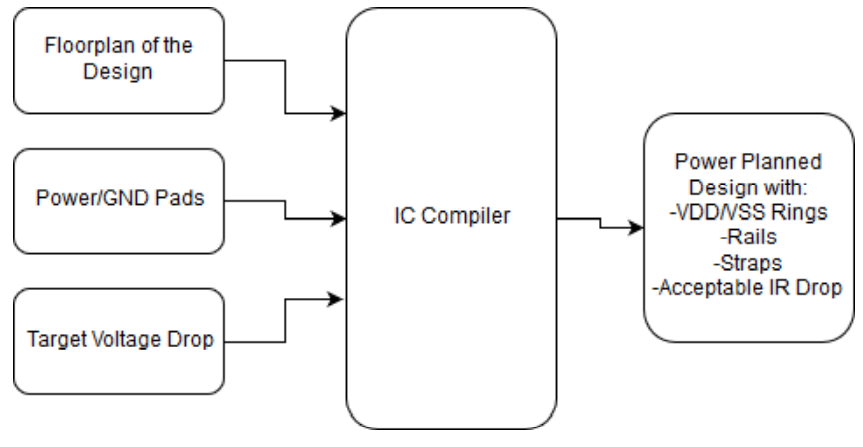
\includegraphics[width=15cm]{diagrams/IO_power.PNG}
\caption{ Inputs and outputs of power-planning}
\label{fig:IO_power}
\end{figure}
%%%%%%%%%%%%%%%%%%%%%%%%%%%%%%%%%%%%%%%%%%%%%%%%%%%%%%%%%%%%%%%%%%%%%%%%%%%%%%%%%%%%%%%%%%%%%%%%%%%%%%
\subsection{Placement}
The placement stage is done using the \textit{place\_opt} command and it has several sub-steps. There are several options for configuring the flow of this stage according to the needs of our design. For example, we may invoke \textit{place\_opt} with \textit{-congestion} to encourage the tool to place cells with the goal of minimizing congestion or with \textit{-area\_recovery} which enables buffer removal and cell downsizing of non critical paths.

\begin{figure}[h]
\centering
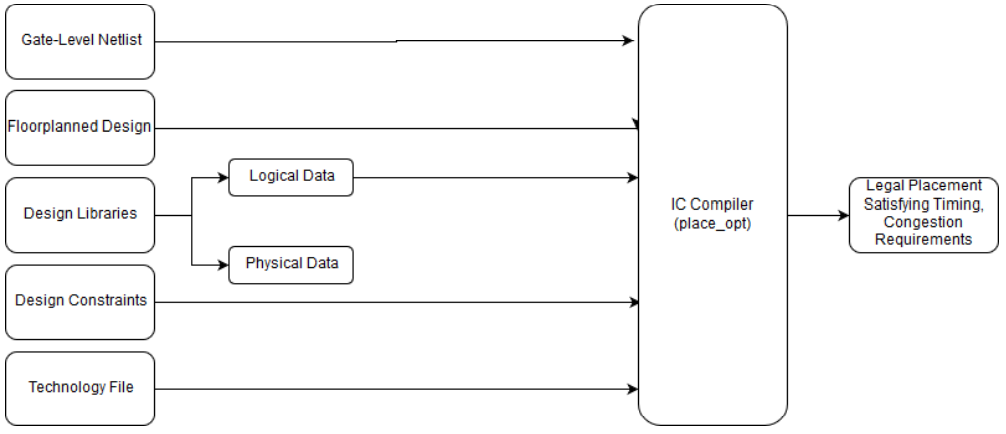
\includegraphics[width=15cm]{diagrams/IO_placment.PNG}
\caption{ Inputs and outputs of the placement stage}
\label{fig:IO_placment}
\end{figure}
%%%%%%%%%%%%%%%%%%%%%%%%%%%%%%%%%%%%%%%%%%%%%%%%%%%%%%%%%%%%%%%%%%%%%%%%%%%%%%%%%%%%%%%%%%%%%%%%%%%%%%
\subsection{Clock Tree Synthesis (CTS)}
The initial state of the design before CTS is as follows:

\begin{enumerate}
\item The placement of the cells of the design should have been completed. 
\item The power and ground nets should have already been pre-routed. 
\item The estimated congestion (from virtual routing) should be acceptable. 
\item The estimated timing should be acceptable (we should have positive or zero slack, we should not be seeing any negative slacks). 
\item The estimated maximum capacitance, transition, etc.. should have no violations. 
\item The high fanout nets should have been synthesized (during AHFS phase in placement as 
discussed above), except for the clock nets. 
\item  The clock nets prior to this stage were treated as ideal and thus will not have been buffered 
so far.\\
Thus before CTS it is assumed that all clock pins are diven by the same clock source 
without any skew.
\end{enumerate}

\begin{figure}[h]
\centering
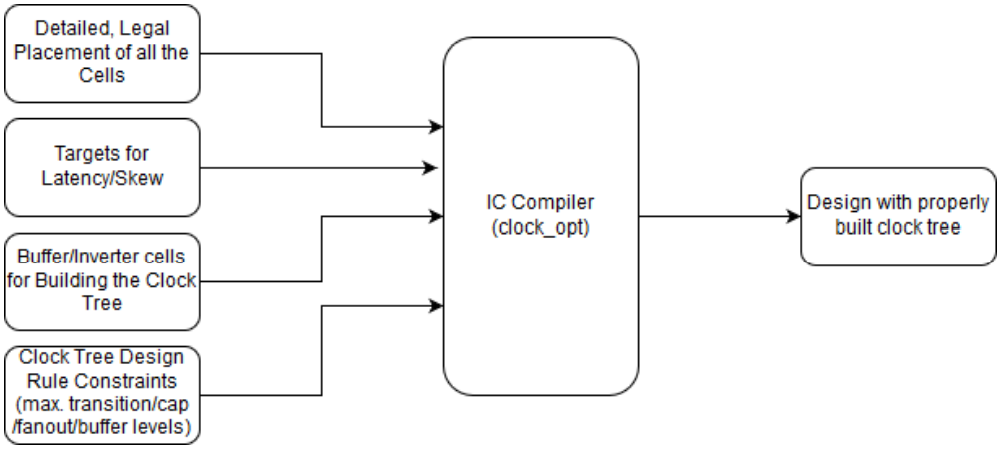
\includegraphics[width=15cm]{diagrams/IO_CTS.PNG}
\caption{ Inputs and outputs of the CTS stage}
\label{fig:IO_CTS}
\end{figure}
%%%%%%%%%%%%%%%%%%%%%%%%%%%%%%%%%%%%%%%%%%%%%%%%%%%%%%%%%%%%%%%%%%%%%%%%%%%%%%%%%%%%%%%%%%%%%%%%%%%%%%
\subsection{Routing}

\begin{enumerate}
\item \textbf{Global Routing:}\\
Global routing (GR) only assigns the nets to be routed to specific metal layers and global routing cells (Gcells). Congestion means that more tracks are needed than available

\item \textbf{Track Assignment:}\\
Assign each net to a specific track and lays down the actual metal traces. This stage also attempts to: make long, straight traces, reduce the number of vias. The Track Assignment does not check or follow physical DRC rules.

\item \textbf{Detail Routing:}\\
Detail route is concerned with specifying the complete interconnect path and fixing all the DRC violations after Track Assignment. The detail router does not work on the entire chip at the same time like Track Assignment. Instead it works by rerouting within the small sub-areas of the design called “SBoxes”

\item \textbf{Search and Repair:}\\
These S\&R loops attempt to fix the remaining DRC violations in the design by working through the design in progressively larger SBoxes. The smaller the SBox, the less routing resources are available to fix the violations but also, the less disruption caused and the less deterioration of timing
\end{enumerate}

\begin{figure}[h]
    \centering
    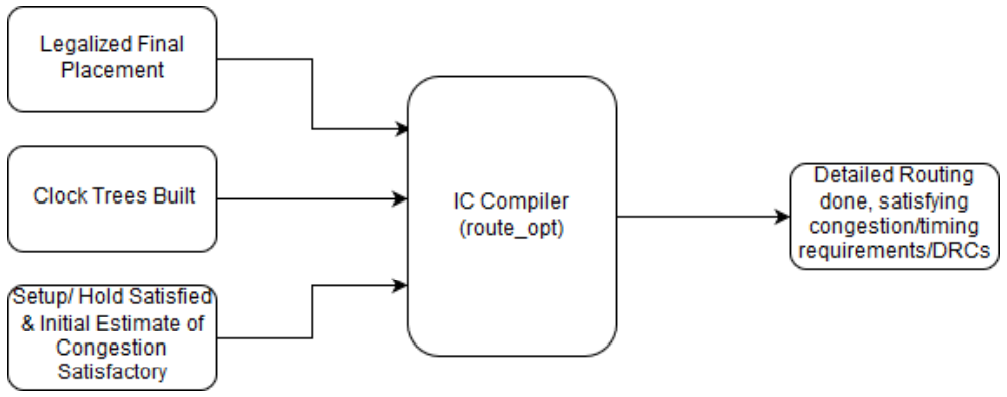
\includegraphics[width=15cm]{diagrams/IO_routing.PNG}
    \caption{ Inputs and outputs of routing}
    \label{fig:IO_routing}
\end{figure}
%%%%%%%%%%%%%%%%%%%%%%%%%%%%%%%%%%%%%%%%%%%%%%%%%%%%%%%%%%%%%%%%%%%%%%%%%%%%%%%%%%%%%%%%%%%%%%%%%%%%%%
\subsection{ RISC-V PnR flow and challenges}
    Add text here
\end{document}
